\section{Results}

All numbers are from the final campaign: 2,268 H1 runs over 108 cells at the
Amendment 2 horizon, 252 H2 runs, 84 H3 runs, and 162 ablation runs over
two operating points, with full manifests released. Two baseline runs
reached congestion collapse at the wall-clock cap and are excluded with
their selection effect disclosed in the readout; the exclusion flatters the
affected baselines and therefore runs against the mechanism.

\subsection{H1: the primary comparison}

\begin{figure*}[tbp]
\centering
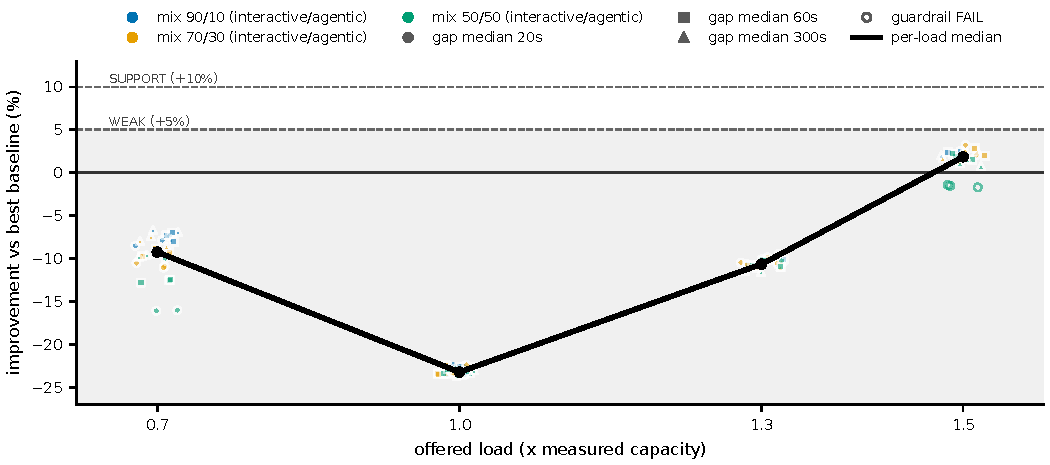
\includegraphics[width=\textwidth]{figures/F1_improvement_vs_load.pdf}
\caption{Per-cell improvement of the reservation discipline over the best per-cell tuned baseline, across offered load. Each point is one of 108 pre-registered core cells; the heavy line traces the per-load median. The deficit is U-shaped, deepest at nominal provisioning (22 to 24 percent at 1.0x), and the sign flips past saturation (+1 to +3 percent at 1.5x). Dashed lines mark the pre-registered WEAK (+5 percent) and SUPPORT (+10 percent) thresholds; no cell reaches SUPPORT. Open symbols mark the three cells failing the interactive guardrail (Section 7.2).}
\label{fig:improvement}
\end{figure*}
\begin{table}[tbp]
\centering
\small
\caption{Pre-registered verdict summary (thresholds fixed 2026-07-06).}
\label{tab:verdict}
\begin{tabular}{llll}
\toprule
threshold & required & measured & outcome \\
\midrule
median improvement & $\geq$ +10\% (support) / $\geq$ +5\% (weak) & -10.3\% & KILL \\
supporting cells & $\geq$ 60\% of core cells & 0 of 108 (0\%) & KILL \\
interactive guardrail & p95 TTFT degradation $\leq$ 5\% & intact in 96\% of cells & holds (4 cells fail) \\
\bottomrule
\end{tabular}

\end{table}

The verdict, computed mechanically against the frozen thresholds:
reservation-based serving loses a median 10.3 percent of goodput per
provisioned GPU-hour to the best per-cell tuned baseline, supports the
hypothesis in 0 of 108 cells against a 60 percent requirement, and holds
the interactive guardrail in 96 percent of cells (Figure 1, Table 2; the
full per-cell table is Appendix D). Under the specification's Section 3,
H1 is killed.

The loss has structure worth more than its median. Across offered load it
is U-shaped (Figure 1): at 0.7x capacity the deficit runs 7 to 16 percent;
at 1.0x it is deepest, 22 to 24 percent in every cell; at 1.3x it recovers
to 9.5 to 11.5 percent; and at 1.5x the sign flips, with reservation ahead
by 0.8 to 3.2 percent in all 24 non-guardrail-failing cells. The deficit
peaks exactly where the cluster is well-provisioned: at nominal load the
work-conserving baselines run at maximum efficiency while reservations
strand capacity across idle gaps, and as load rises past saturation the
baselines begin to thrash while stranding matters relatively less, until
the ordering inverts at the top of the region. Completion guarantees, on
this evidence, are most expensive precisely when the fleet is sized
correctly.

The other axes are quieter. Cluster size is nearly flat: 8-, 16-, and
32-device cells agree within roughly a point throughout, which bears on
the Amendment 3 scope reduction, since nothing in the measured trend
suggests the removed 64-device axis behaves categorically differently.
Idle-gap distribution has a mild, consistent effect: longer gap medians
shrink the deficit at low load (at 50/50 mix and 0.7x load, the loss is
16 percent at 20-second gaps but 9.5 percent at 300-second gaps), because
longer gaps favor the tiered-pin embodiment's spill-and-restore over
holding hot capacity. At three seeds the paired bootstrap intervals are
tight and solidly negative in the load 1.0 band, wider at 0.7x where
several upper bounds cross zero; the verdict does not depend on any cell
whose interval is ambiguous, since zero cells reach the support threshold
under any reading.

\subsection{What the stranding buys: isolation, and where it inverts}

\begin{figure*}[tbp]
\centering
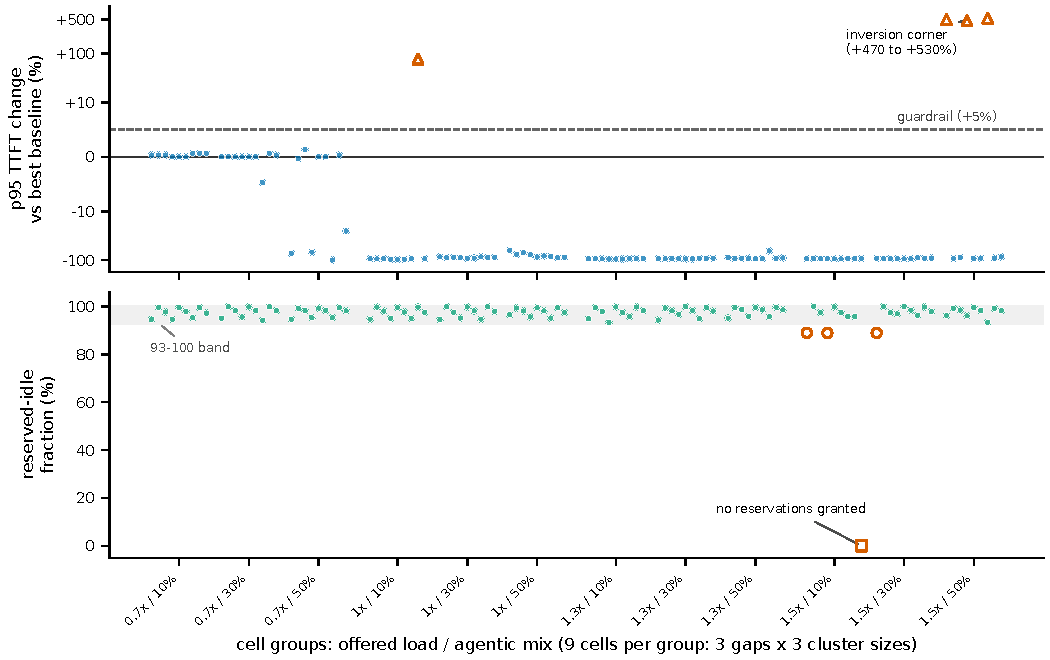
\includegraphics[width=\textwidth]{figures/F2_isolation_and_stranding.pdf}
\caption{What the stranding buys. (a) Interactive p95 time-to-first-token change versus the best baseline per cell: at and above nominal load, reservations improve interactive tail latency by 63 to 97 percent by keeping agentic flows off the shared pool; the effect inverts only in the heavy-agentic, overloaded, short-gap corner, where the guardrail fails (Section 7.2). (b) Reserved-idle fraction per cell: the isolation of panel (a) is priced in capacity held idle, 93 to 100 percent of the reserved pool in 77 of 81 cells, with three load-1.5 cells at 88.9 percent and one cell granted no reservations (marked), the structural duty-cycle cost of Section 7.5.}
\label{fig:ledger}
\end{figure*}

The guardrail was pre-registered as a constraint, interactive p95
time-to-first-token degraded no more than 5 percent, and the mechanism did
not merely satisfy it: in most of the region it inverted it. At and above
nominal load, reservations improve interactive tail latency by 63 to 97
percent relative to the best baseline, above 90 percent in most such
cells, while reserved-idle fraction runs 93 to 100 percent in 77 of 81 such
cells (Figure 2; three load-1.5 cells sit at 88.9 percent, admission
having granted few reservations there, and one cell is degenerate at
zero, admission having granted none).
Read together with Section 7.1, this is the ledger's purchase side made
precise: the 9.5 to 23.6 percent goodput deficit buys near-order-of-magnitude
tail-latency protection for interactive traffic, by structurally keeping
long flows off the shared pool. Operators who price interactive tail
latency highly are buying exactly this, and today they buy it by
overprovisioning; the discipline prices the same isolation in stranded
capacity instead.

The purchase fails in one measured corner. At heavy agentic mix, overload,
and short gaps (50/50, 1.5x, 20-second gaps), the guardrail fails
spectacularly, interactive p95 TTFT worse by roughly 470 to 530 percent
across all three cluster sizes. The mechanism is legible: with half the
token volume agentic, gaps short enough that reserved flows cycle almost
continuously, and offered load half again over capacity, the reserved
subset occupies the machine and interactive traffic starves on the
residue. Isolation, in other words, is a property of the regime, not of
the mechanism, and it reverses exactly where reservations are densest and
the machine is most oversubscribed. One further isolated failure (90/10
mix, nominal load, 8 devices, 300-second gaps, against a FastServe
baseline, +77 percent) does not repeat at any neighboring cell.

\subsection{H2: the graceful-degradation hypothesis, reversed and killed}

\begin{figure}[tbp]
\centering
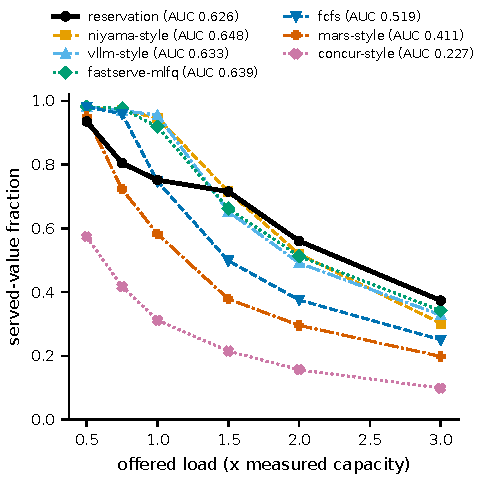
\includegraphics[width=3.4in]{figures/F3_served_value.pdf}
\caption{Served value across the load sweep. The reservation discipline's area under curve (0.626) trails deterministic demotion (0.648), killing the graceful-degradation hypothesis; the admission-throttling baselines collapse under overload (Section 7.3).}
\label{fig:servedvalue}
\end{figure}

H2 held that degradation keyed to committed headroom yields a better
served-value curve under overload than deterministic demotion and
preempt-and-requeue. It does not. Over the full load sweep (0.5x to 3.0x),
the reservation discipline's served-value area under curve is 0.626
against the best baseline's 0.648 (Niyama-style deterministic demotion), a
3.4 percent deficit; FastServe and vLLM-style also finish ahead (Figure
3). H2 carries only corrected-horizon data: an earlier censored-horizon
reading was ruled unverified and excluded from the released record, and
Section 8 explains why censored-horizon comparisons mislead; the
superseded preliminary readouts are released as filed. Two
baselines collapse under overload on this metric, the MARS-style admission
controller (0.411) and CONCUR-style AIMD (0.227), both of which protect
the system by throttling intake and pay for it in served value. The
mechanism's load-1.5 sign flip in Section 7.1 and its H2 loss are
consistent, not contradictory: past saturation the discipline completes
more valued flows per provisioned hour while shedding best-effort work
hard enough to lose on aggregate served value.

\subsection{H3: containment, and the starvation result}

\begin{figure}[tbp]
\centering
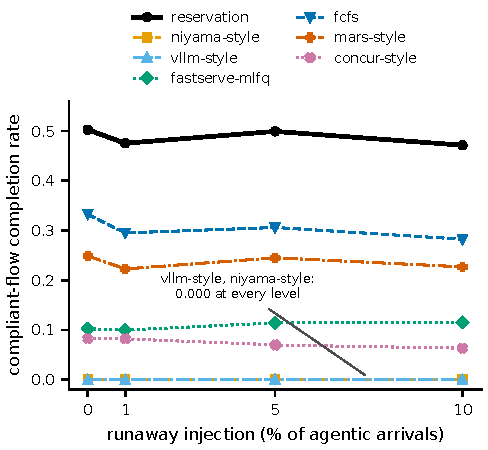
\includegraphics[width=3.4in]{figures/F4_containment_starvation.pdf}
\caption{Compliant-flow completion under adversarial runaway injection, absolute rates. The reservation discipline holds near 0.5 with a worst-case degradation of 3.1 points; FCFS completes 0.33 with no containment; the two strongest request-oriented baselines complete zero compliant flows at every level including no injection, instrumented admission starvation (one of 107 compliant flows ever scheduled, zero preemptions; Section 7.4). Deltas against zero are undefined, which is why rates are absolute.}
\label{fig:containment}
\end{figure}
\begin{table}[tbp]
\centering
\footnotesize
\caption{H3 absolute compliant-flow completion rates at each runaway-injection level, with the worst delta versus the no-injection condition (percentage points).}
\label{tab:h3}
\begin{tabular}{lrrrrr}
\toprule
policy & inj 0\% & inj 1\% & inj 5\% & inj 10\% & worst delta \\
\midrule
reservation & 0.503 & 0.475 & 0.499 & 0.471 & -3.1 \\
fcfs & 0.332 & 0.295 & 0.306 & 0.282 & -5.0 \\
mars\_style & 0.249 & 0.223 & 0.245 & 0.227 & -2.6 \\
fastserve\_mlfq & 0.102 & 0.100 & 0.114 & 0.116 & -0.3 \\
concur\_style & 0.082 & 0.082 & 0.070 & 0.063 & -1.9 \\
vllm\_style & 0.000 & 0.000 & 0.000 & 0.000 & +0.0 \\
niyama\_style & 0.000 & 0.000 & 0.000 & 0.000 & +0.0 \\
\bottomrule
\end{tabular}

\end{table}

Under adversarial runaway injection at 0, 1, 5, and 10 percent of agentic
arrivals, the discipline's cross-invocation budget does what it was
specified to do: compliant-flow completion holds at 0.503, 0.475, 0.499,
and 0.471, a worst-case degradation of 3.1 points, and every runaway is
cut off at exactly its budget (Figure 4, Table 3). The comparison column,
however, is the finding. The two strongest request-oriented baselines,
vLLM-style and Niyama-style, complete 0.000 of compliant agentic flows at
every injection level including zero. This is not a missing measurement;
it is instrumented starvation. At the H3 configuration (50/50 mix, 1.2x
load), those policies schedule 1 of 107 compliant agentic flows, with
zero preemptions: under interactive-class priority, long flows simply
never receive a device slot while interactive traffic saturates the
cluster, and the result is locked by a regression test. A delta against
zero is undefined, which is why this table reports absolute rates.
Section 2 argued that a flow can be under budget and starved at the same
time, and that a scheduler can be locally optimal at every step while
starving the flow; Section 4.2 argued that priorities are not contracts;
this table is both arguments, measured. FCFS, blind to class, completes
0.332 and degrades 5.0 points under injection: no isolation, no
containment, but no starvation either. The discipline is the only policy
in the set that is simultaneously above 0.3 absolute and below 3.5 points
of adversarial degradation.

\subsection{Ablations: which element carries the cost}

The ablation campaign removes one element at a time from the tuned
discipline, nine variants at three mixes and three seeds, at two operating
points: an uncontended nominal-load cell, and a contended cell with four
times the decode slots, 1.3x load, and the grid's shortest gaps, chosen
because the binding analysis of Section 7.6 shows the memory and
peak-decode constraints demonstrably engage there. We report the campaign's
result as its own noise analysis forces us to: across both operating
points, no element of the discipline shows an effect on the primary metric
distinguishable from seed noise. At the contended cell, the total goodput
spread across all nine variants is 0.68 percent, against a within-variant
seed spread whose median is 29 percent; at the nominal cell the two spreads
are the same order of magnitude. One apparent effect appeared and did not
survive: at the nominal cell, replacing headroom-keyed degradation with
queue-depth keying improved goodput by 20.9 percent, but the effect
vanished at the contended cell (+0.2 percent) and sits within the nominal
cell's own seed spread; an earlier internal readout called it corroborating
evidence, and that reading is withdrawn in the released, corrected
document. With three seeds, a per-element median is a draw from a
distribution wider than the effects being measured, and this design cannot
separate an inert element from an unexercised one; per-element attribution
needs swept load and slot axes and materially more replications, and the
per-run data is released for exactly that. This noise floor is a property
of the ablation design, not of the primary comparison: H1's per-cell
deltas are paired, every policy scoring byte-identical workload
realizations, which cancels the workload draw that dominates the unpaired
within-variant spread here, and the H1 verdict is additionally invariant
to interval readings, since zero cells reach the support threshold under
any of them.

What the campaign does establish is robust because it is large and
consistent rather than a difference between near-identical numbers:
reserved capacity sits 88 to 95 percent idle at both operating points,
despite the contended cell's quadrupled slots, elevated load, and minimal
gaps. The reason is structural. An agentic flow runs a short invocation and
then waits in tool time, a duty cycle of roughly 5 percent by
construction, so capacity reserved for such flows is stranded nine parts
in ten regardless of configuration, and no variant in either cell recovers
the loss. The ablation campaign's honest conclusion is that the
mechanism's cost is not located in any single element; it is located in
the duty cycle of the workload the mechanism reserves for. Section 4.2
presented the forward-looking commitment signal as a design claim; at the
operating points tested here, no advantage of that signal over queue depth
is attributable above the noise floor, and the system-level H2 comparison
of Section 7.3 is negative. The tuning campaign's independent,
cross-family K-to-floor result (Section 5), the optimizer choosing the
smallest reserved subset offered in every workload family at both
horizons, points the same way at larger scale.

\subsection{Sensitivity: what the numbers are conditioned on}

\begin{table}[tbp]
\centering
\footnotesize
\caption{Service-model sensitivity: measured effect and binding classification per constant.}
\label{tab:sens}
\begin{tabular}{llll}
\toprule
constant & perturbation & representative-cell delta & binding \\
\midrule
single-stream decode rate & 0.7x / 1.3x & deficit 21.5\% $\to$ 4.4\% / 13.0\% & binding \\
peak decode rate & $\pm$30\% & none (0 of 19{,}342 decode calls bound) & non-binding \\
cache bytes per token & $\pm$30\% & none (peak HBM near 39\% of capacity) & non-binding \\
\bottomrule
\end{tabular}

\end{table}

Service-model constants are literature-anchored estimates, and the
evaluation measured which ones matter (Table 4). The single-stream decode
rate is the binding constant, and it is material: at 0.7x the anchored
value, the representative cell's deficit compresses from 21.5 to 4.4
percent; at 1.3x it is 13.0 percent. The sign of the verdict is robust
across the tested range; the magnitude is genuinely uncertain at roughly
the factor the anchor is uncertain, and we state this as the paper's
principal fidelity caveat, unresolvable here because the hardware phase
was gated on this evaluation's outcome and the gate closed. Two further
constants, peak decode rate and cache bytes per token, do not move the
representative cell's result at all, and the released binding analysis
shows why, with instrumentation rather than assertion: at 16 decode slots
the batch is capped below the size at which peak decode can bind (0 of
19,342 decode calls), and peak memory occupancy stays near 39 percent of
capacity, so a 30 percent perturbation changes no placement decision. At
a deliberately memory-bound configuration (64 slots, agentic-heavy, 1.5x
load), both constants demonstrably bind (peak decode governs 43 percent
of calls, memory saturates), confirming the harness detects binding where
binding exists and that the main grid's device configuration sits in the
compute-bound regime. Regression tests pin all three properties.
